% Switch this line to the final option when submitting your thesis.
% This will correct counts and remove labels that are shown during draft mode
\documentclass[masters,draft]{UTPAthesis}
%\documentclass[masters,final]{UTPAthesis}
%\documentclass[masters,final, nodedication, noacknowledgments]{UTPAthesis}


%% Load your packages below.
%% Make hyperref and showkeys come at the end of your loaded packages
%% to make sure they are not over-written.  They redefine many
%% standard LaTeX commands
\usepackage{booktabs} % for better tables
\usepackage[colorlinks=false]{hyperref}  % for urls
\usepackage{showkeys} % this is a convenient package, but causes problems



% Insert your name and major here in the format shown
\Author{John Q. Citizen}
\AuthorLastFirst{Citizen, John Q.}
\Major{Mathematics}


% Insert your graduation date here
\Month{May}
\Year{2014}


% Insert the title of your thesis here.
% If you have a long title, split it between multiple lines using the \\ command
% Also, use comment characters to avoid unwanted spaces in the Abstract page
\Title{Titles Should Not Exceed Six Inches on One Line\\
   and In The Inverted Pyramid Format\\
   When Additional Lines Are Needed%
}


% Insert your research advisor and his title here
\Advisor{Dr. Leonhard Euler}
\AdvisorTitle{Chair of Committee}


%% Insert the members of your committee here
\MemberA{Dr. Carl Friedrich Gauss}  %\MemberATitle{Co-Chair of Committee}
\MemberB{Dr. G. F. Bernhard Riemann}
\MemberC{}
\MemberD{}


% Insert the text of your abstract below.
% The thesis manual also requires a bibliography style "citation" here.
% Insert the counts for tables and figures.
\Abstract{%
  An abstract is a brief summary often used to help the reader quickly
  ascertain the paper's purpose.
}


% You can dedicate your paper here
\Dedication{%
Dedication should be simple, in good taste, and fit on one page.
}


% Acknowledge those who helped and supported you here.
\Acknowledgments{%
Acknowledgements should be simple, in good taste, and fit on one page.
}


% Insert your biographical sketch here.
\BiographicalSketch{%
A brief biographical sketch of the student is required as part of each thesis.
}



\begin{document}

% This starts page counting in Roman numerals
\frontmatter


% This command makes the formal preliminary pages.
% You can comment it out during the drafting process if you want to save paper.
\makepreliminarypages


% These insert a table of contents, list of tables, and list of figures
\tableofcontents
\listoftables
\listoffigures


% This starts regular page counting in Arabic numerals
\mainmatter

% This starts double-spaced text.  Opposite command is \singlespace
\doublespace


% OK. Everything is set up. Insert your thesis below.
% It's a good idea to split your thesis up into different files and use
% the \input command
\chapter{Introduction}

In Synthetic Aperture Radar (SAR) imaging, radar antennas are mounted on an airborne or spaceborne platform. The scene to be imaged is illuminated by electromagnetic waves transmitted from an antenna. The goal is to extract information of the scene from the measurements taken of the scattered waves.

\section{Blah Blah}


Many of the principles of SAR imaging are applicable to other fields such as
acoustics, geophysics, and medical imaging. In particular, it has been shown
that spotlight-mode SAR can be described as a tomographic reconstruction problem
and can be analyzed using the projection slice theorem from computer-aided
tomography\cite{Garza:2011fk}

\begin{equation}\label{eq:einstein}
	e = mc^{2}
\end{equation}



\begin{figure}
  \centering
  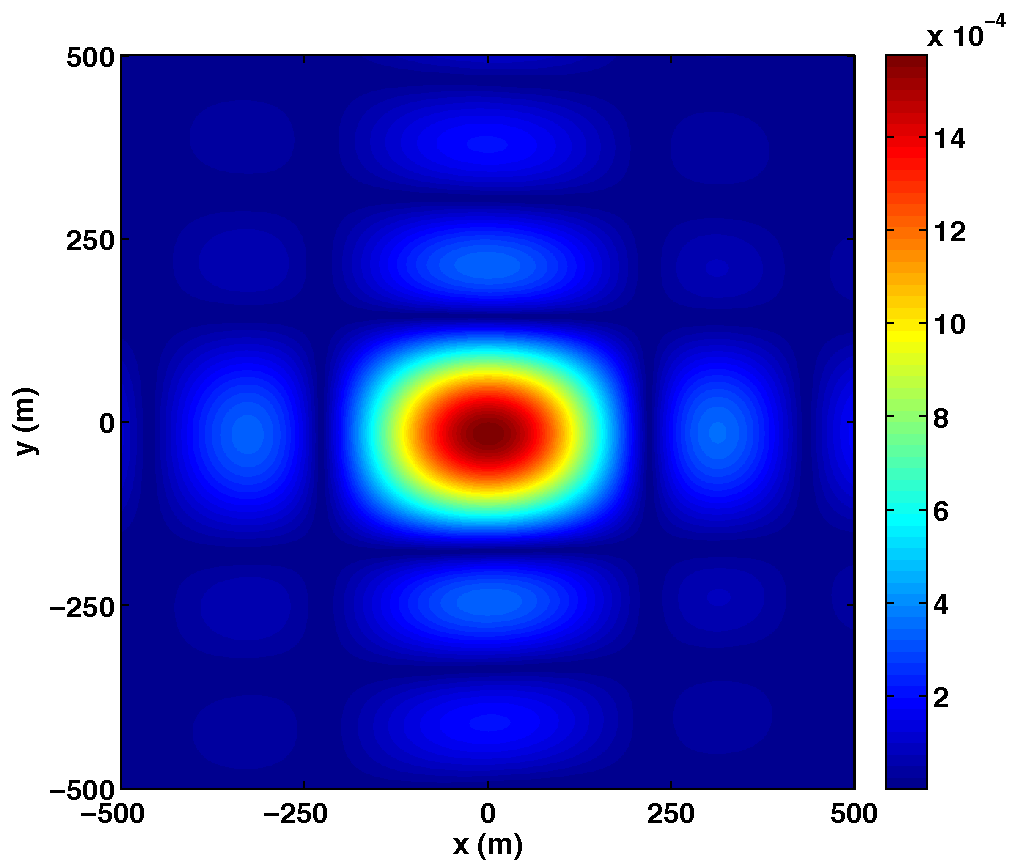
\includegraphics[scale=0.5]{figures/beamfootprint}
  \caption[Colorful Picture]{This is a colorful picture.}
  \label{fig:flyover}
\end{figure}




%  Uncomment the following line for appendixes
%\appendix


% This makes the bibliography.
% Enter your references in the BibTex file "references.bib"
% You can find bibtex info from Google Scholar.
\bibliographystyle{siam}
\bibliography{references}


% This inserts your Biographical Sketch
\biographypage

\end{document}
